\documentclass[a4paper,12pt]{article}

% Paquetes básicos
\usepackage[utf8]{inputenc}
\usepackage[T1]{fontenc}
\usepackage[spanish]{babel}
\usepackage{graphicx}
\usepackage{xcolor}
\usepackage{lipsum}
\usepackage{geometry}
\geometry{top=3cm, bottom=3cm, left=2.5cm, right=2.5cm}

% Paquetes para diseño
\usepackage{titlesec}
\usepackage{fancyhdr}
\usepackage{amsmath}
\usepackage{amssymb}
\usepackage{hyperref}

% Paquetes para el entorno lstlisting
\usepackage{listings}
\usepackage{inconsolata}

%encabezado y pie de página nivel profesional
\usepackage{fancyhdr}
\pagestyle{fancy}
\fancyhf{}
\fancyhead[L]{\leftmark}
\fancyhead[R]{\rightmark}
\fancyfoot[C]{\thepage}
\fancyfoot[R]{\textbf{(UGR)} \today}
\renewcommand{\headrulewidth}{0.4pt}
\renewcommand{\footrulewidth}{0.4pt}
\setlength{\headheight}{15pt}
\setlength{\headsep}{10pt}
\setlength{\footskip}{20pt}
\usepackage{truncate}
\fancyhead[L]{\truncate{0.5\headwidth}{\leftmark}}
\fancyhead[R]{\truncate{0.5\headwidth}{\rightmark}}
\usepackage{mathpazo}
% Paquete para fondo
\usepackage{background}

% Configuración de lstlisting
\lstset{
    inputencoding=utf8,          % Permite UTF-8
    extendedchars=true,          % Reconoce caracteres extendidos
    literate=                    % Configuración manual para tildes y símbolos
        {á}{{\'a}}1
        {é}{{\'e}}1
        {í}{{\'i}}1
        {ó}{{\'o}}1
        {ú}{{\'u}}1
        {ñ}{{\~n}}1
        {Á}{{\'A}}1
        {É}{{\'E}}1
        {Í}{{\'I}}1
        {Ó}{{\'O}}1
        {Ú}{{\'U}}1
        {Ñ}{{\~N}}1
        {¿}{{\textquestiondown}}1
        {¡}{{\textexclamdown}}1,
    basicstyle=\ttfamily,        % Fuente monoespaciada
    breaklines=true,             % Habilita salto de línea automático
    frame=single,                % Marco alrededor del código
    backgroundcolor=\color{gray!10}, % Fondo gris claro
    keywordstyle=\color{blue},   % Color para palabras clave
    commentstyle=\color{green},  % Color para comentarios
    stringstyle=\color{red}      % Color para strings
}
\lstdefinestyle{customcpp}{
    language=C++,                % Lenguaje de programación
    showspaces=false,            % No mostrar espacios
    showtabs=false,              % No mostrar tabulaciones
    tabsize=4,                   % Tamaño de tabulación
    showstringspaces=false,      % No mostrar espacios en strings
    numbers=left,                % Números de línea a la izquierda
    numberstyle=\tiny\color{gray}, % Estilo de los números de línea
    numbersep=5pt,               % Separación de los números de línea
    stepnumber=1,                % Mostrar número en cada línea
    basicstyle=\ttfamily\footnotesize, % Estilo básico del código
    keywordstyle=\bfseries\color{blue}, % Estilo de las palabras clave
    commentstyle=\itshape\color{green!50!black}, % Estilo de los comentarios
    stringstyle=\color{red},     % Estilo de los strings
    identifierstyle=\color{black}, % Estilo de los identificadores
    % procnamekeys={def,class},    % Palabras clave para nombres de funciones
    morekeywords={constexpr,nullptr,size_t}, % Más palabras clave
    emph={int,char,double,float,unsigned}, % Palabras a enfatizar
    emphstyle=\color{magenta},   % Estilo de las palabras enfatizadas
    backgroundcolor=\color{gray!10}, % Color de fondo
    frame=shadowbox,             % Marco con sombra
    rulesepcolor=\color{gray},   % Color de la línea de separación
    breakatwhitespace=false,     % No cortar en espacios en blanco
    breaklines=true,             % Cortar líneas largas
    captionpos=b,                % Posición del título (abajo)
    escapeinside={(*@}{@*)},     % Delimitadores para escapar a LaTeX
    morecomment=[l][\color{magenta}]{\#}, % Comentarios de una línea
    morecomment=[s][\color{orange}]{/*}{*/}, % Comentarios multilínea
    morestring=[b]",             % Strings entre comillas dobles
    morestring=[b]'              % Strings entre comillas simples
}

% Configuración de título
\titleformat{\section}{\normalfont\Large\bfseries}{\thesection}{1em}{}

% Información del documento
\title{
    \vspace{-2cm}
    
\includegraphics[width=0.3\textwidth]{images/etsiit.png} \\ % Cambia el logo si es necesario
    \LARGE Ingeniería Informática + ADE\\
    \large Universidad de Granada (UGR)\\[1cm]
}
\author{\textbf{Autor:} Ismael Sallami Moreno}
\date{\textbf{Asignatura:} Ejercicios Tema 3 SCD: Paso de mensajes}

% Configuración del fondo
\backgroundsetup{
    scale=1,
    color=black,
    opacity=0.2,
    angle=0,
    position=current page.south,
    vshift=0pt,
    hshift=0pt,
    contents={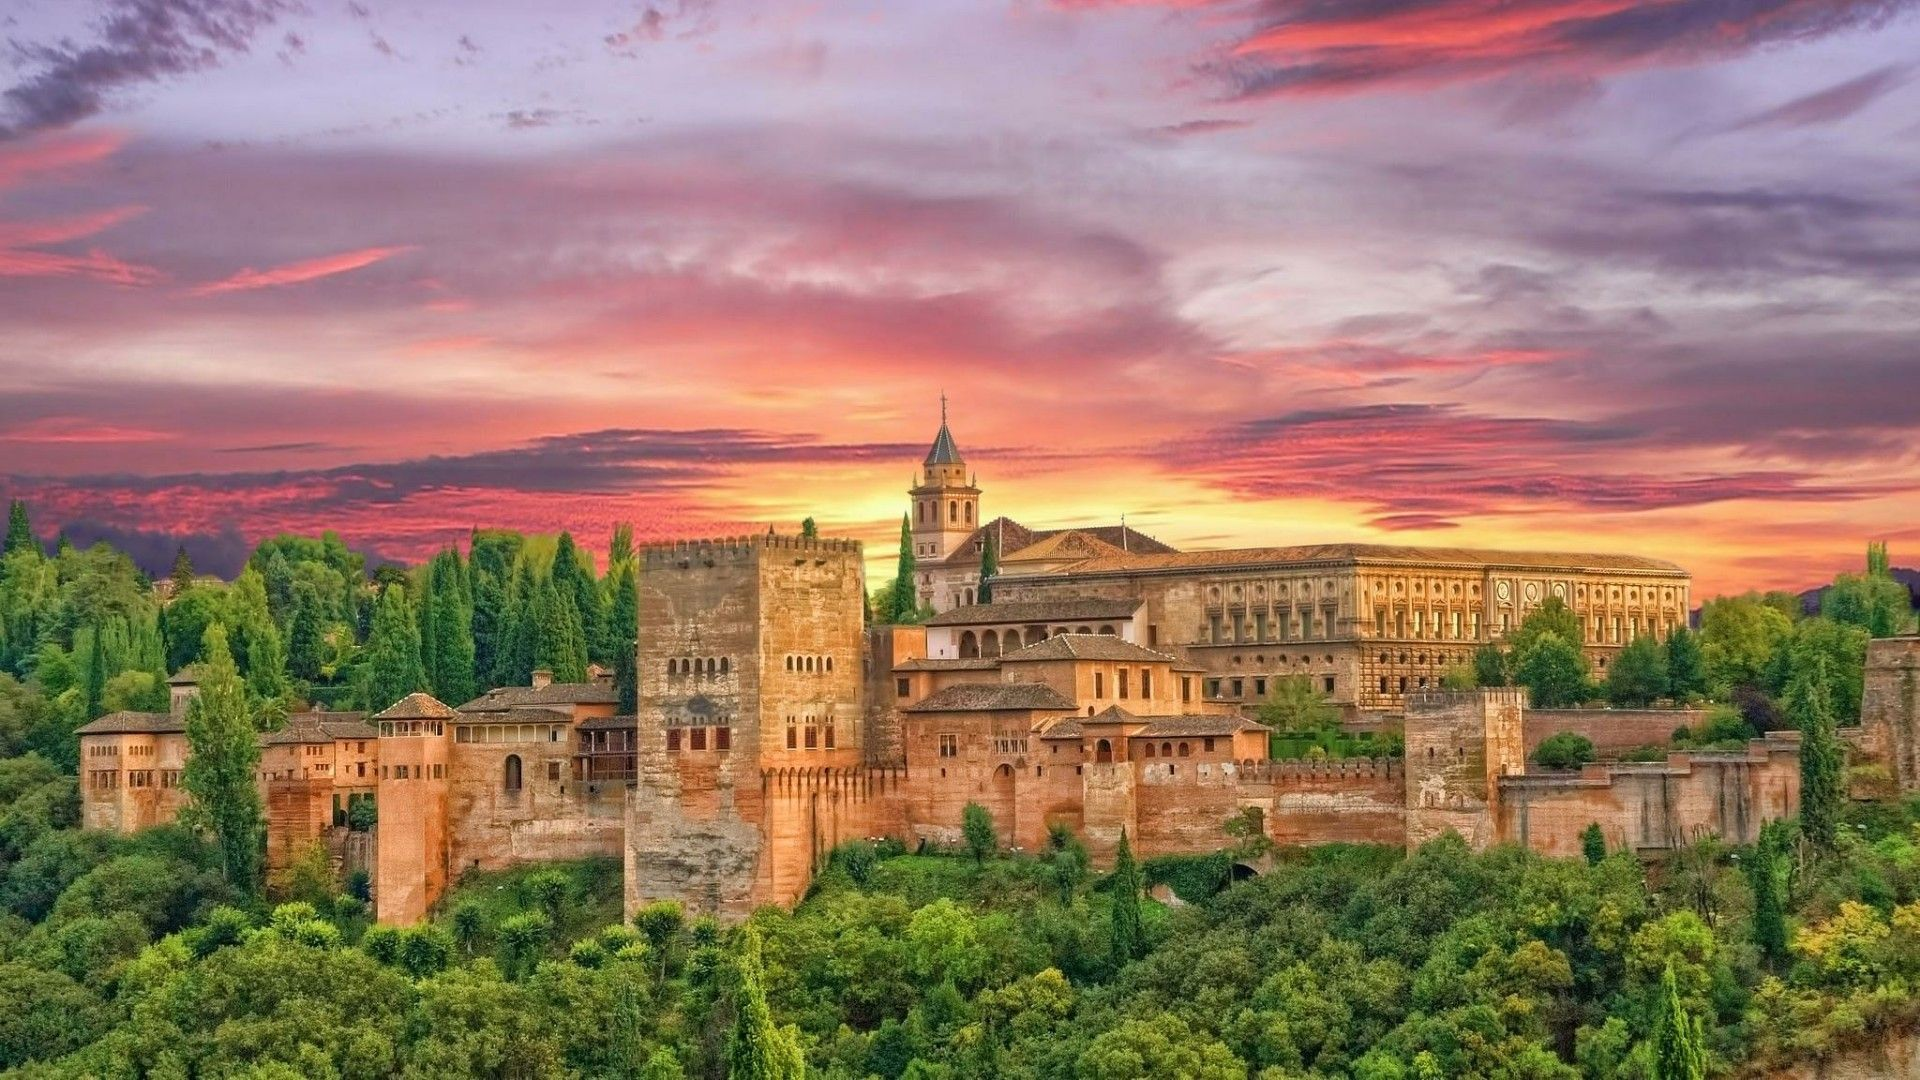
\includegraphics[width=\paperwidth,height=\paperheight,keepaspectratio]{images/granada.jpg}}
}

% Inicio del documento
\begin{document}

% Portada
\maketitle
\thispagestyle{empty}

\begin{center}
    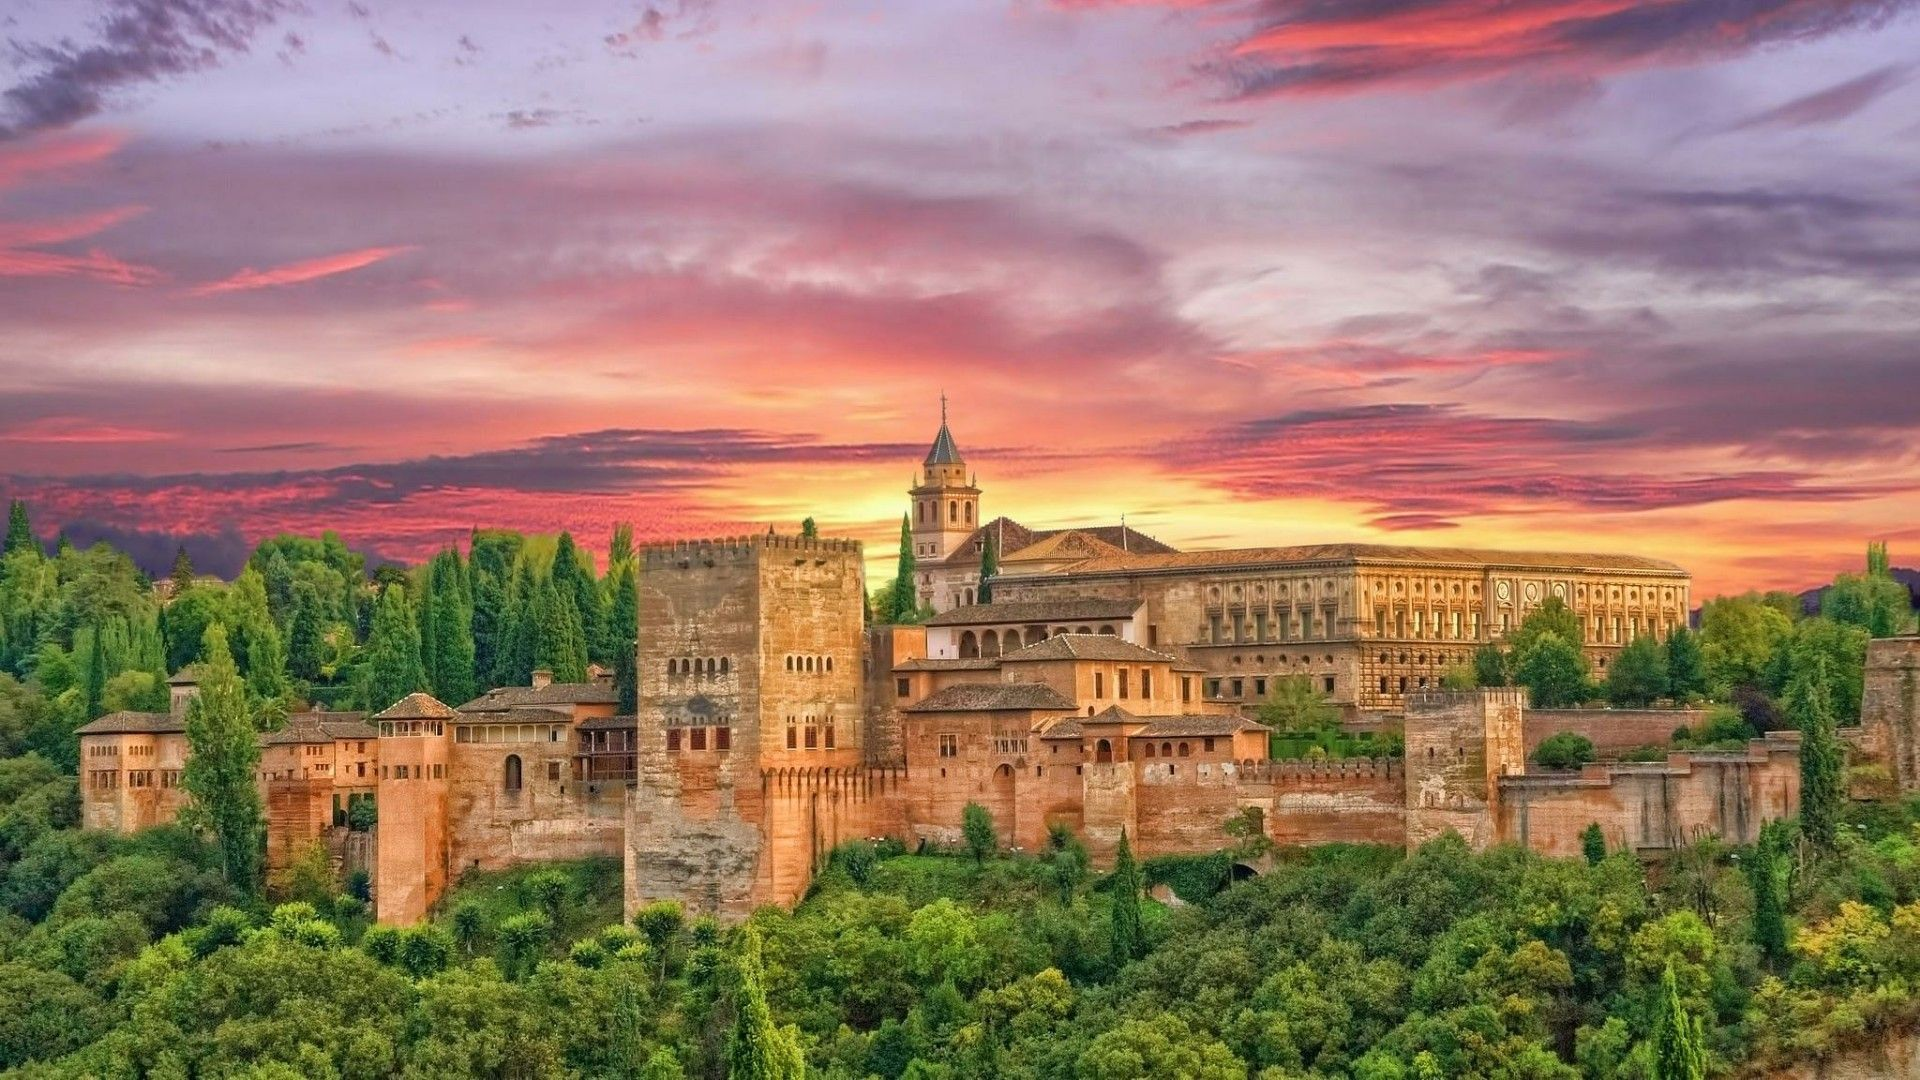
\includegraphics[width=\textwidth,height=0.4\textheight,keepaspectratio]{images/granada.jpg} \\ % Añade tu imagen de fondo
    \vfill
\end{center}

\newpage

% Índice (opcional)
\tableofcontents
\newpage
\section{Ejercicio 77}

\subsection{Enunciado}
En un sistema distribuido, 6 procesos clientes necesitan sincronizarse de forma específica para
realizar cierta tarea, de forma que dicha tarea sólo podrá ser realizada cuando tres procesos estén
preparados para realizarla. Para ello, envían peticiones a un proceso controlador del recurso y
esperan respuesta para poder realizar la tarea específica. El proceso controlador se encarga
de asegurar la sincronización adecuada. Para ello, recibe y cuenta las peticiones que le llegan
de los procesos, las dos primeras no son respondidas y producen la suspensión del proceso
que envía la petición (debido a que se bloquea esperando respuesta) pero la tercera petición
produce el desbloqueo de los tres procesos pendientes de respuesta. A continuación, una vez
desbloqueados los tres procesos que han pedido (al recibir respuesta), inicializa la cuenta y
procede cíclicamente de la misma forma sobre otras peticiones. El código de los procesos
clientes aparece aquí abajo. Los clientes usan envío asíncrono seguro para realizar su petición,
y esperan con una recepción síncrona antes de realizar la tarea:

\begin{lstlisting}[style=customcpp]
process Cliente[ i : 0..5 ] ;
begin
  while true do begin
    send( peticion, Controlador );
    receive( permiso, Controlador );
    Realiza_tarea_grupal();
  end
end

process Controlador ;
begin
  while true do begin
    ...
  end
end
\end{lstlisting}

Describir en pseudocódigo el comportamiento del proceso controlador, utilizando una orden de
espera selectiva que permita implementar la sincronización requerida entre los procesos. Es
posible utilizar una sentencia del tipo select for i=... to ... para especificar diferentes ramas de una sentencia selectiva que comparten el mismo código dependiente del valor
de un índice i.

\subsection{Solucion}

En un sistema distribuido, 6 procesos clientes necesitan sincronizarse de forma específica para realizar cierta tarea, de forma que dicha tarea sólo podrá ser realizada cuando tres procesos estén preparados para realizarla. Para ello, envían peticiones a un proceso controlador del recurso y esperan respuesta para poder realizar la tarea específica. El proceso controlador se encarga de asegurar la sincronización adecuada. 

El controlador cuenta las peticiones que le llegan de los procesos:
\begin{itemize}
    \item Las dos primeras peticiones no son respondidas, lo que provoca que los procesos que las envían queden bloqueados esperando una respuesta.
    \item La tercera petición produce el desbloqueo de los tres procesos pendientes, enviándoles una respuesta.
\end{itemize}

Una vez desbloqueados los tres procesos, el controlador inicializa la cuenta y procede cíclicamente de la misma forma para nuevas peticiones. Los clientes usan envío asíncrono seguro para realizar su petición y esperan con una recepción síncrona antes de realizar la tarea.

El código de los procesos clientes es el siguiente:

\begin{lstlisting}[style=customcpp, caption={Código de los procesos clientes}]
process Cliente[ i : 0..5 ] ;
begin
  while true do begin
    send( peticion, Controlador );   // Envía una petición al proceso controlador.
    receive( permiso, Controlador ); // Espera un permiso del controlador.
    Realiza_tarea_grupal();         // Realiza la tarea grupal una vez recibido el permiso.
  end
end
\end{lstlisting}

El comportamiento del proceso controlador, que asegura la sincronización, se describe en pseudocódigo a continuación:

\begin{lstlisting}[style=customcpp, caption={Pseudocódigo del proceso Controlador}]
process Controlador ;
var
  contador : integer := 0;           // Cuenta las peticiones recibidas.
  buffer : array[0..2] of integer;   // Almacena los índices de los procesos en espera.

begin
  while true do begin
    select
      for i := 0 to 5                // Itera sobre las peticiones de los procesos clientes.
      when receive( peticion, Cliente[i] ) do
        buffer[contador] := i;       // Almacena el índice del proceso cliente en el buffer.
        contador := contador + 1;    // Incrementa el contador de peticiones.

        if contador = 3 then begin   // Si se han recibido tres peticiones...
          for j := 0 to 2 do
            send( permiso, Cliente[buffer[j]] ); // Envía permiso a los tres procesos.
          contador := 0;             // Reinicia el contador.
        end
    end
  end
end
\end{lstlisting}

\textbf{Explicación del código del controlador:}
\begin{itemize}
    \item El proceso controlador mantiene un contador de peticiones y un buffer que almacena los índices de los clientes en espera.
    \item Por cada petición recibida, almacena el índice del cliente en el buffer y aumenta el contador.
    \item Cuando el contador alcanza tres, el controlador envía permisos a los tres procesos almacenados en el buffer y reinicia el contador.
\end{itemize}

Este enfoque asegura que los clientes se sincronizan correctamente antes de realizar la tarea grupal, tal como se requiere en el enunciado.



\end{document}
